\section{Experiments}
\label{sec:experiments}

\subsection{Datasets}
We used several subsets of Imagenet~\cite{deng2009imagenet} for training and evaluation of our methods. We also evaluate a 
tracking
algorithm on a video of scuba divers taken from Youtube \footnote{https://www.youtube.com/watch?v=QmRFmhILd5o}. Subsets of 
Imagenet
containing underwater images were selected for the training of CycleGAN, and manually separated into two classes based on visual
inspection. We let $X$ be the set of underwater images with no distortion, and $Y$ be the set of underwater images with 
distortion. $X$
contained 6143 images, and $Y$ contained 1817 images. We then trained CycleGAN to learn the mapping $F: X \rightarrow Y$, such 
that images
from $X$ appeared to have come from $Y$. Finally, our image pairs for training data were generated by distorting all images in $X$ 
with
$F$. Figure~\ref{fig:cgan_samples} shows sample training pairs. When comparing with CycleGAN, we used a test set of 56 images 
acquired from
Flickr\texttrademark .

\subsection{Evaluation}
We train UGAN and UGAN-P on the image pairs generated by CycleGAN, and evaluate on the images from the
test set, $Y$. Note that these images do not contain any ground truth, as they are original distorted images from
Imagenet. Images for training and testing are of size $256 \times 256 \times 3$ and normalized between $[-1, 1]$.
Figure ~\ref{fig:test_samples} shows samples from the test set. Notably, these images contain varying amounts of noise. Both UGAN 
and UGAN-P
are able to recover lost color information, as well as correct any color information this is present. 

While many of the distorted images contain a blue or green hue over the entire image space, that is not always the case.
In certain environments,
it is possible that objects close to the camera are undistorted with correct colors, while the background
of the image contains distortion. In these cases, we would like the network to only correct parts of the image that
appear distorted. The last row in Figure ~\ref{fig:test_samples} shows a sample of such an image. The orange of the clownfish is 
left
unchanged while the distorted sea anemone in the background has its color corrected.

For a quantitative evaluation we compare to CycleGAN, as it inherently learns an inverse mapping during the training of
$G: Y \rightarrow X$. We first use the Canny edge detector
\cite{canny1986computational}, as this provides a color agnostic evaluation of the images in comparison to ground truth.
Second, we compare local image patches to provide sharpness metrics on our images. Lastly, we show how an existing
tracking algorithm for an underwater robot improves performance with generated images.

\begin{figure}
\centering
\begin{tabular}{p{1.7cm} p{1.7cm} p{1.7cm}}

   ~\quad Original & ~\quad \textbf{UGAN} & \quad \textbf{UGAN-P} \\

   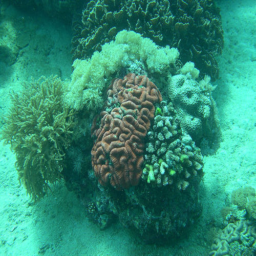
\includegraphics[width=0.8in]{n01917289_4982_real} &
   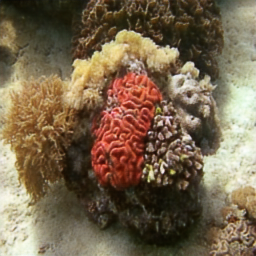
\includegraphics[width=0.8in]{n01917289_4982_gen_0} &
   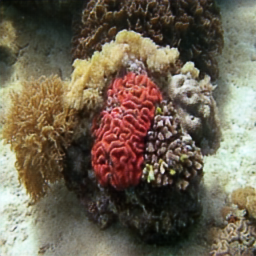
\includegraphics[width=0.8in]{n01917289_4982_gen_1} \\

   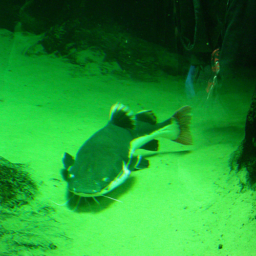
\includegraphics[width=0.8in]{n01496331_16340_real} &
   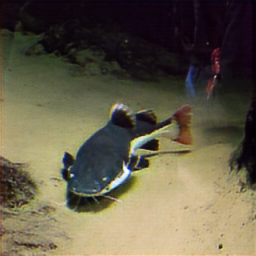
\includegraphics[width=0.8in]{n01496331_16340_gen_0} &
   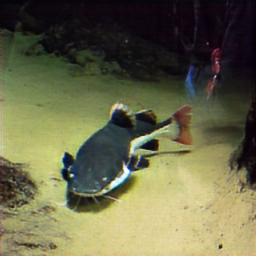
\includegraphics[width=0.8in]{n01496331_16340_gen_1} \\
   
   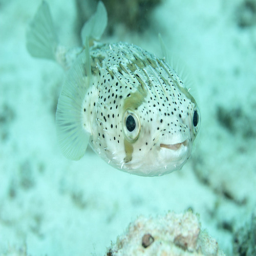
\includegraphics[width=0.8in]{n01496331_22183_real} &
   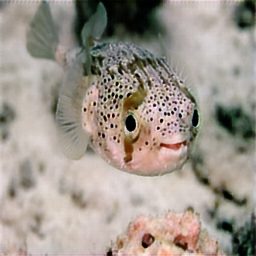
\includegraphics[width=0.8in]{n01496331_22183_gen_0} &
   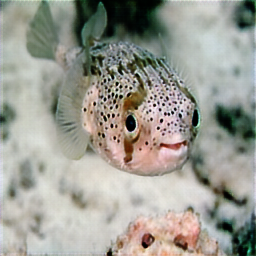
\includegraphics[width=0.8in]{n01496331_22183_gen_1} \\
   
   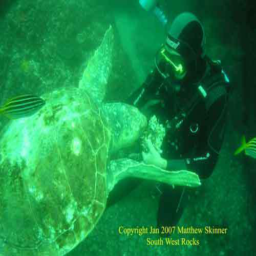
\includegraphics[width=0.8in]{n01664065_29738_real} &
   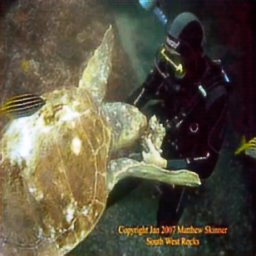
\includegraphics[width=0.8in]{n01664065_29738_gen_0} &
   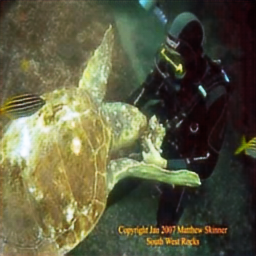
\includegraphics[width=0.8in]{n01664065_29738_gen_1} \\
   
   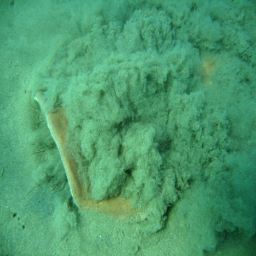
\includegraphics[width=0.8in]{n01496331_11938_real} &
   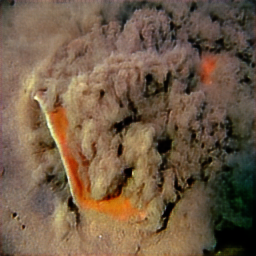
\includegraphics[width=0.8in]{n01496331_11938_gen_0} &
   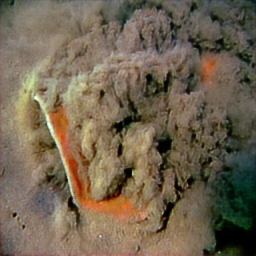
\includegraphics[width=0.8in]{n01496331_11938_gen_1} \\
   
   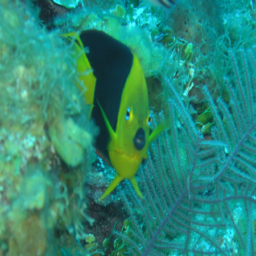
\includegraphics[width=0.8in]{n02606052_2969_real} &
   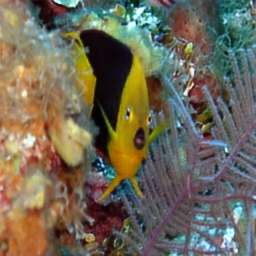
\includegraphics[width=0.8in]{n02606052_2969_gen_0} &
   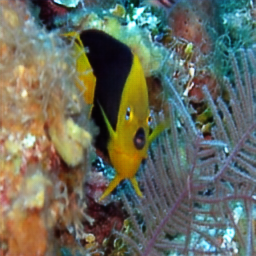
\includegraphics[width=0.8in]{n02606052_2969_gen_1} \\
   
   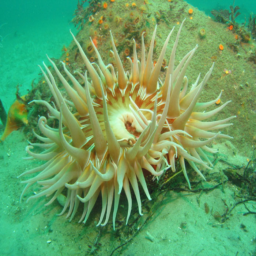
\includegraphics[width=0.8in]{n01914609_1607_real} &
   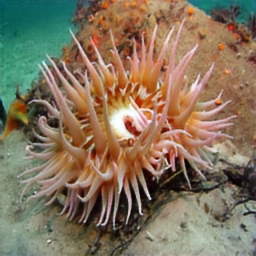
\includegraphics[width=0.8in]{n01914609_1607_gen_0} &
   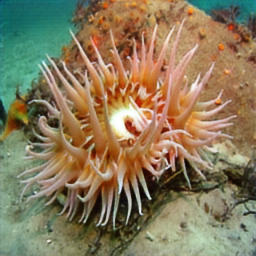
\includegraphics[width=0.8in]{n01914609_1607_gen_1} \\

   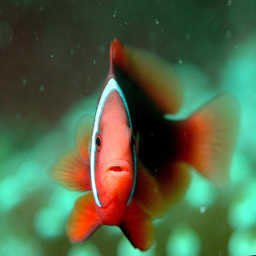
\includegraphics[width=0.8in]{n02607072_6241_real} &
   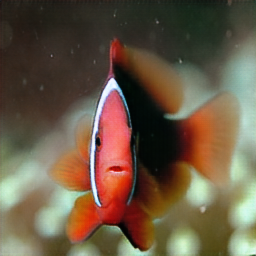
\includegraphics[width=0.8in]{n02607072_6241_gen_0} &
   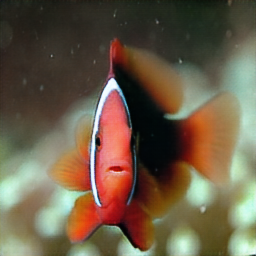
\includegraphics[width=0.8in]{n02607072_6241_gen_1} \\

\end{tabular}
\caption{Samples from our Imagenet testing set. The network can both recover color and also correct color if a small amount is 
present.}
\label{fig:test_samples}
\end{figure}

% Directly from the first paper on the inception score: We find that it’s important to evaluate the metric on a large
% enough number of samples (i.e. 50k) as part of this metric measures diversity.
% % Therefore we should not include it I think
% \footnote{Code for inception score can be found at https://github.com/openai/improved-gan}
%\begin{center}
%\begin{tabular}{c c c c c c}
%Samples & real & ugan & ugan-p & cyclegan \\ \hline
%Model & True Images & UGAN & UGAN-P & CycleGAN \\ \hline
%Score $\pm$ std. & $5.69 \pm 0.23$ & $6.18 \pm 0.35$ & $6.30 \pm 0.32$ & $6.37 \pm 0.43$ \\ \hline
%\end{tabular}
%\end{center}


\subsection{Training and Inference Performance}
In all of our experiments, we use $\lambda_{1} = 100$, $\lambda_{GP} = 10$, batch size of 32, and the Adam Optimizer 
\cite{kingma2014adam} with learning rate $1e-4$. Following WGAN-GP, the discriminator is updated $n$ times for every update of the 
generator, where $n = 5$. For UGAN-P, we set $\lambda_{2} = 1.0$ and $\alpha = 1$. Our implementation was done using the 
Tensorflow library \cite{abadi2016tensorflow}. \footnote{Code is available at 
\url{https://github.com/cameronfabbri/Underwater-Color-Correction}} All networks were trained from scratch on a GTX 1080 for 100 
epochs. Inference on the GPU takes on average $ 0.0138s$, which is about 72 Frames Per Second (FPS). On a CPU (Intel Core 
i7-5930K), inference takes on average $ 0.1244s$, which is about 8 FPS. We find both of these measures acceptable for underwater 
tasks.

\subsection{Comparison to CycleGAN}
It is important to note that during the process of learning a mapping $F: X \rightarrow Y$, CycleGAN also learns a
mapping $G: Y \rightarrow X$. Here we give a comparison to our methods. We use the Canny edge
detector \cite{canny1986computational} to provide a color agnostic evaluation of the images, as the original contain
distorted colors and cannot be compared back to as ground truth. Due to the fact that restoring color information
should not alter the overall structure of the image, we measure the distance in the image space between the edges
found in the original and generated images. Figure ~\ref{fig:canny_samples} shows the original images and results from
edge detection. Table 1 provides the measurements from Figure ~\ref{fig:canny_samples}, as well as the average over our
entire Flickr\texttrademark ~dataset. Both UGAN and UGAN-P are consistently closer in the image space to the original
than that of CycleGAN, suggesting noise due to blur. Next, we evaluate this noise explicitly.

We explore the artifacts of content loss, as seen in Figure ~\ref{fig:zoom}. In particular, we compare local statistics
of the highlighted image patches, where each image patch is resized to $64 \times 64$. We use the GDL
\cite{mathieu2015deep} from (\ref{gdl_eq}) as a sharpness measure. A lower GDL measure implies a smoother transition
between pixels, as a noisy image would have large jumps in the image's gradient, leading to a higher score. \starnote{I THINK. I would double check, bottom of page 4: https://arxiv.org/pdf/1511.05440.pdf}.
As seen in Table \ref{fig:gdl_tbl}, the GDL is lower for both UGAN and UGAN-P. Interestingly, UGAN consistently has a
lower score than UGAN-P, despite UGAN-P explicitly accounting for this metric in the objective function. Reasoning for
this is left for our future work.

Another metric we can use to compare image patches are the mean and standard deviation of a patch. The standard
deviation gives us a sense of blurriness because it defines how far the data deviates from the mean. A lower standard
deviation means that the data is closer to the mean \starnote{not sure if we exactly need to say that because I assume the reviewers will know what it is}. In the case of images, this would suggest a blurring effect due to the data being
more clustered toward one pixel value. Table \ref{fig:mean_tbl} shows the mean and standard deviations for the local
image patches seen in Figure \ref{fig:zoom}. Despite qualitative evaluation showing our methods are much sharper,
quantitatively they show only slight improvement. Other metrics such as entropy are left as future work.

% I would like this table to match up with the figure showing edge detections. I wasn't able to
% get letters on the left side at each row though.
\begin{table}
\centering
\caption{Distances in image space}
\begin{tabular}{| c | c | c | c |}
   \hline
   Row/Method & CycleGAN & \textbf{UGAN} & \textbf{UGAN-P} \\ \hline
   A          & 116.45 & 85.71  & 86.15  \\ \hline
   B          & 114.49 & 97.92  & 101.01 \\ \hline
   C          & 120.84 & 96.53  & 97.57  \\ \hline
   D          & 129.27 & 108.90 & 110.50 \\ \hline
   Mean       & 111.60 & 94.91  & 96.51 \\ \hline
\end{tabular}
\end{table}

%\newpage

\begin{figure}
\centering
\begin{tabular}{p{1.7cm} p{1.7cm} p{1.7cm} p{1.7cm}}
  
   ~\quad Original & ~CycleGAN & ~\quad \textbf{UGAN} & \quad \textbf{UGAN-P} \\

   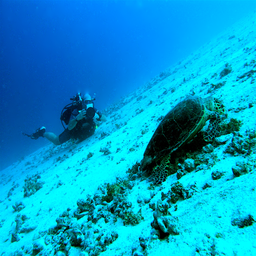
\includegraphics[width=0.8in]{1_original} &
   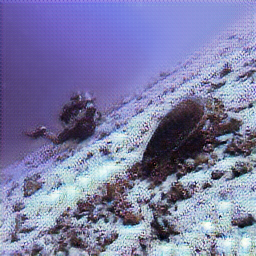
\includegraphics[width=0.8in]{1_cimg} &
   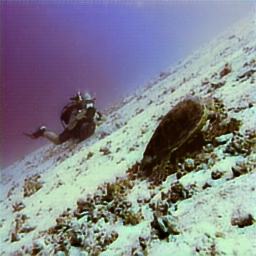
\includegraphics[width=0.8in]{1_u0img} &
   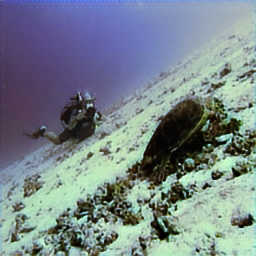
\includegraphics[width=0.8in]{1_u1img} \\ [-1ex]
   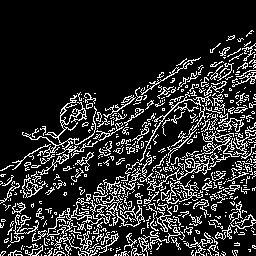
\includegraphics[width=0.8in]{1_oedges} &
   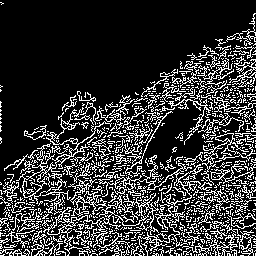
\includegraphics[width=0.8in]{1_cedges} &
   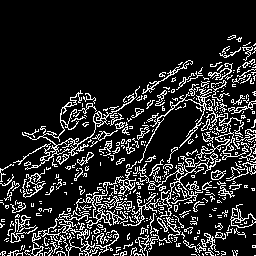
\includegraphics[width=0.8in]{1_u0edges} &
   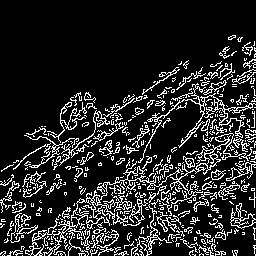
\includegraphics[width=0.8in]{1_u1edges} \\

   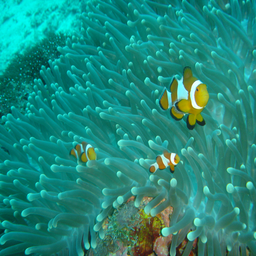
\includegraphics[width=0.8in]{2_original} &
   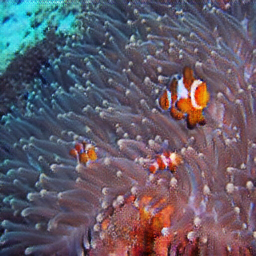
\includegraphics[width=0.8in]{2_cimg} &
   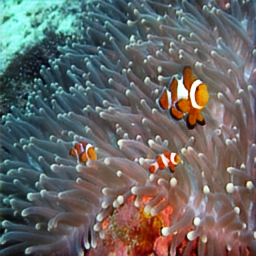
\includegraphics[width=0.8in]{2_u0img} &
   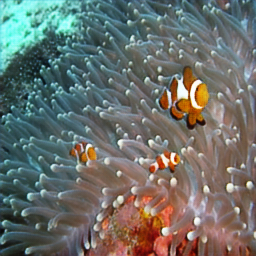
\includegraphics[width=0.8in]{2_u1img} \\ [-1ex]
   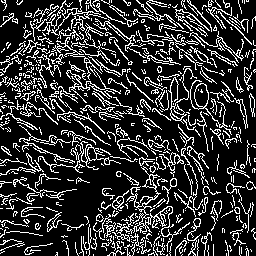
\includegraphics[width=0.8in]{2_oedges} &
   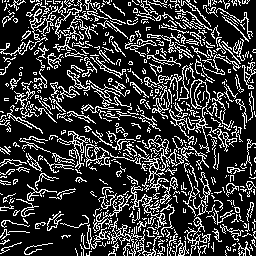
\includegraphics[width=0.8in]{2_cedges} &
   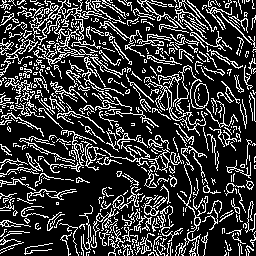
\includegraphics[width=0.8in]{2_u0edges} &
   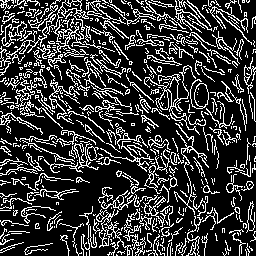
\includegraphics[width=0.8in]{2_u1edges} \\

   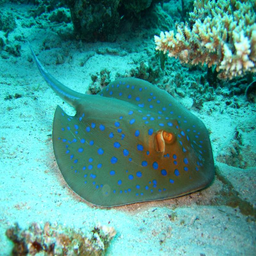
\includegraphics[width=0.8in]{3_original} &
   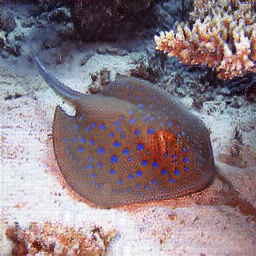
\includegraphics[width=0.8in]{3_cimg} &
   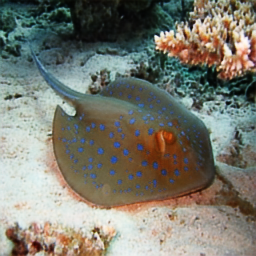
\includegraphics[width=0.8in]{3_u0img} &
   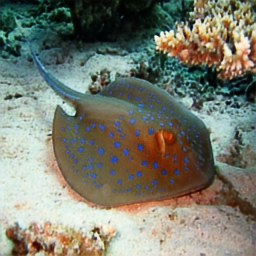
\includegraphics[width=0.8in]{3_u1img} \\ [-1ex]
   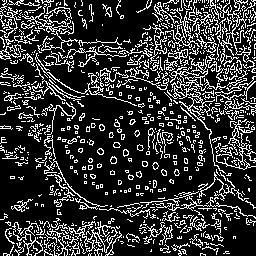
\includegraphics[width=0.8in]{3_oedges} &
   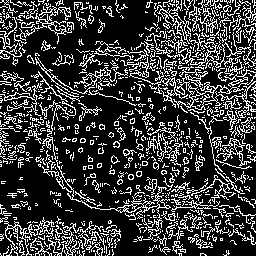
\includegraphics[width=0.8in]{3_cedges} &
   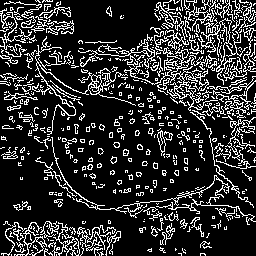
\includegraphics[width=0.8in]{3_u0edges} &
   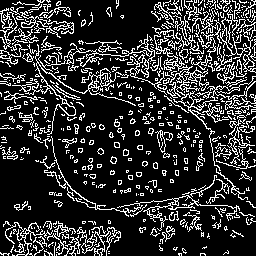
\includegraphics[width=0.8in]{3_u1edges} \\
   
   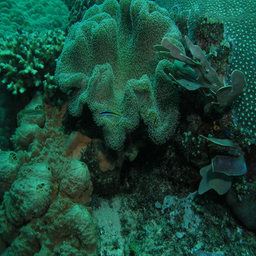
\includegraphics[width=0.8in]{4_original} &
   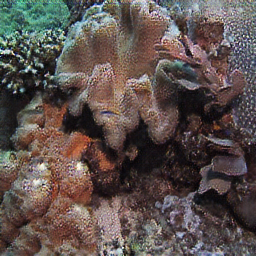
\includegraphics[width=0.8in]{4_cimg} &
   \includegraphics[width=0.8in]{4_u0img} &
   \includegraphics[width=0.8in]{4_u1img} \\ [-1ex]
   \includegraphics[width=0.8in]{4_oedges} &
   \includegraphics[width=0.8in]{4_cedges} &
   \includegraphics[width=0.8in]{4_u0edges} &
   \includegraphics[width=0.8in]{4_u1edges} \\

\end{tabular}
\caption{Running the Canny Edge Detector on sample images. Both variants of UGAN contain less noise than CycleGAN,
and are closer in the image space to the original. For each pair, the top row is the input image, and bottom row
the result of the edge detector.}
\label{fig:canny_samples}
\end{figure}

% TODO definitely need help with formatting, but content is there
\begin{figure*}
\centering
\begin{tabular}{p{4.0cm} p{4.0cm} p{4.0cm} p{4.0cm}}
  
   \qquad \qquad ~ Original & \qquad \qquad CycleGAN & \qquad \qquad ~ \textbf{UGAN} & \qquad \qquad \textbf{UGAN-P} \\

   \includegraphics[width=1.7in]{flickr_cmp} &
   \includegraphics[width=1.7in]{cgan_cmp} &
   \includegraphics[width=1.7in]{ugan_cmp} &
   \includegraphics[width=1.7in]{uganp_cmp} \\ [-2ex]
   
\end{tabular}
\end{figure*}

\begin{figure*}
\begin{tabular}{p{1.8cm} p{1.85cm} p{1.8cm} p{1.8cm} p{1.8cm} p{1.8cm} p{1.8cm} p{1.9cm} }
   
   \includegraphics[width=0.8in]{flickr_crop1} &
   \includegraphics[width=0.8in]{flickr_crop2} &
   \includegraphics[width=0.8in]{cgan_crop1} &
   \includegraphics[width=0.8in]{cgan_crop2} &
   \includegraphics[width=0.8in]{ugan_crop1} &
   \includegraphics[width=0.8in]{ugan_crop2} &
   \includegraphics[width=0.8in]{ugan_crop1} &
   \includegraphics[width=0.8in]{ugan_crop2} \\

   \includegraphics[width=0.8in]{flickr_crop3} &
   \includegraphics[width=0.8in]{flickr_crop4} &
   \includegraphics[width=0.8in]{cgan_crop3} &
   \includegraphics[width=0.8in]{cgan_crop4} &
   \includegraphics[width=0.8in]{ugan_crop3} &
   \includegraphics[width=0.8in]{ugan_crop4} &
   \includegraphics[width=0.8in]{ugan_crop3} &
   \includegraphics[width=0.8in]{ugan_crop4} \\

\end{tabular}
\caption{Comparison of local image patches. Each patch was resized to $64 \times 64$.}
\label{fig:zoom}
\end{figure*}

\begin{table}[ht]
\footnotesize
\centering
\caption{Gradient Difference Loss Metrics}
\begin{tabular}{| c | c | c | c | }
   \hline
   Patch/Method & CycleGAN & \textbf{UGAN} & \textbf{UGAN-P} \\ \hline
   Red    & 11.53 & 9.39 & 10.93  \\ \hline
   Blue   & 7.52  & 4.83 &  5.50\\ \hline
   Green  & 4.15  & 3.18 & 3.25 \\ \hline
   Orange & 6.72  & 5.65 & 5.79 \\ \hline
\end{tabular}
\label{fig:gdl_tbl}
\end{table}

\begin{table}[ht]
\footnotesize
\centering
\caption{Mean and Standard Deviation Metrics}
\begin{tabular}{| c | c | c | c | c | }
   \hline
   Patch/Method & Original & CycleGAN & \textbf{UGAN} & \textbf{UGAN-P} \\ \hline
   Red & 0.43 $\pm$ 0.23 & 0.42 $\pm$ 0.22 & 0.44 $\pm$ 0.23 & 0.45 $\pm$ 0.25 \\ \hline
   Blue & 0.51 $\pm$ 0.18 & 0.57 $\pm$ 0.17 & 0.57 $\pm$ 0.17 & 0.57 $\pm$ 0.17 \\ \hline
   Green & 0.36 $\pm$ 0.17 & 0.36 $\pm$ 0.14 & 0.37 $\pm$ 0.17 & 0.36 $\pm$ 0.17 \\ \hline
   Orange & 0.3 $\pm$ 0.15 & 0.25 $\pm$ 0.12 & 0.26 $\pm$ 0.13 & 0.27 $\pm$ 0.14 \\ \hline
\end{tabular}
\label{fig:mean_tbl}
\end{table}

\subsection{Diver Tracking using Frequency-Domain Detection}
We investigate the frequency-domain characteristics of the restored images through a case-study of periodic motion tracking in 
sequence of images. Particularly, we compared the performance of Mixed Domain Periodic Motion (MDPM)- tracker 
\cite{islam2017mixed} on a sequence of images of a diver swimming in  arbitrary directions. MDPM tracker is designed for 
underwater robots to follow scuba divers by   tracking distinct frequency-domain signatures (high-amplitude spectra at $1$-$2$Hz) 
pertaining to human swimming. Amplitude spectra in frequency-domain correspond to the periodic intensity variations in image-space 
over time, which is often eroded in noisy underwater images \cite{shkurti2017underwater}.

Fig. \ref{mdpmStuff} illustrates the improved performance of MDPM tracker on generated images compared to the real ones. 
Underwater images often fail to capture the true contrast in intensity values between foreground and background due to low 
visibility. The generated images seem to restore these eroded intensity variations to some extent, causing much improved positive 
detection for MDPM tracker.

\begin{figure*}
\centering
\begin{tabular}{p{4.0cm} p{4.0cm} p{4.0cm} p{4.0cm}}
   \includegraphics[width=1.7in]{mdpm/real1} &
   \includegraphics[width=1.7in]{mdpm/real2} &
   \includegraphics[width=1.7in]{mdpm/real3} &
   \includegraphics[width=1.7in]{mdpm/real4} \\
   \includegraphics[width=1.7in]{mdpm/gen1} &
   \includegraphics[width=1.7in]{mdpm/gen2} &
   \includegraphics[width=1.7in]{mdpm/gen3} &
   \includegraphics[width=1.7in]{mdpm/gen4} \\
\end{tabular}
\label{fig:mdpm}
\vspace{4mm}

\begin{tabular}{l|c|c|c|r|}
 \cline{2-5}
 &  Correct detection & Wrong detection & Missed detection & Total \# of frames\\ \hline  \cline{2-4}
On real images  &  42 & 14 & 444 & 500  \\ \hline
On generated images  &  147 & 24 & 329 & 500  \\ \hline
\end{tabular}

\caption{Performance of MDPM tracker \cite{islam2017mixed} on both real (top row) and generated (second row) images; the Table 
compares the detection performance for both sets of images over a sequence of $500$ frames.   }
\label{mdpmStuff}
\end{figure*}


%Flippers of a human diver typically oscillate at frequencies between $1$ and $2$ Hz, which produces periodic intensity variations 
in the image-space over time. These variations correspond to distinct signatures in the frequency-domain (high-amplitude spectra 
at $1$-$2$Hz), which can be used for reliable detection.
